\PassOptionsToPackage{unicode}{hyperref}
\documentclass[aspectratio=1610, captions=tableheading, 9pt]{beamer}
\usepackage{booktabs}
% Load packages you need here
\usepackage{polyglossia}
\setmainlanguage{german}

\usepackage{csquotes}
    

\usepackage{amsmath}
\usepackage{amssymb}
\usepackage{mathtools}
\usepackage[mathrm=sym]{unicode-math}

\usepackage[
  locale=DE,                 % deutsche Einstellungen
  separate-uncertainty=true, % immer Fehler mit \pm
  per-mode=reciprocal,       % ^-1 für inverse Einheiten
  % alternativ:
  % per-mode=reciprocal, % m s^{-1}
  % decimal-marker=., % . statt , f�r Dezimalzahlen
]{siunitx}

\usepackage{hyperref}
\usepackage{bookmark}
\usepackage[utf8]{inputenc}

% load the theme after all packages

\usetheme[
  showtotalframes, % show total number of frames in the footline
]{tudo}

% Put settings here, like
\unimathsetup{
  math-style=ISO,
  bold-style=ISO,
  nabla=upright,
  partial=upright,
  mathrm=sym,
}

\usepackage{tikz-feynman}
\usepackage{xfrac}

% nur wenn akkurat auf dem Rechner installiert ist:
\setsansfont{Akkurat Light}[
  BoldFont=Akkurat Bold,
]


\author[J. Alameddine]{Jean-Marco Alameddine}
\title{Implementation von Myon-Paarproduktion in PROPOSAL}
\date[12.02.2019]{12.02.2019}

\institute[%
  {\includegraphics[height=\headerheight]{e5b.pdf}}%
]{E5b}

%\titlegraphic{\includegraphics[height=0.4\textheight]{example-image-a}}

\begin{document}

\begin{frame}
  \maketitle
\end{frame}


\begin{frame}{Prozess der Myon-Paarproduktion}
  \begin{columns}
    \column{0.5\textwidth}
    \begin{center}
      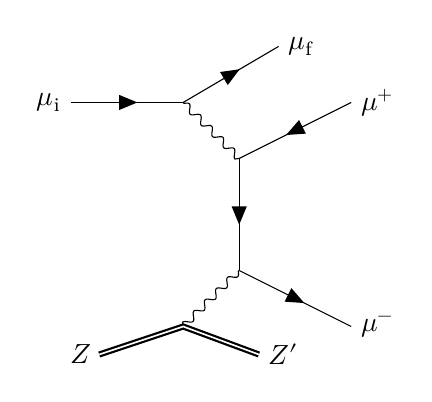
\begin{tikzpicture}
      \centering
       % Sizes
       \pgfmathsetmacro{\len}{0.05cm}
       \pgfmathsetmacro{\halflen}{\len/4}
       \pgfmathsetmacro{\vertexsize}{\len/20}
       \begin{feynman}
           % vertices
           \vertex (a) at (0, 0);
           \vertex (b) at (0, -1*\len);
           \vertex (d) at (-0.5*\len, 0.5*\len);
           \vertex (c) at (-0.5*\len, -1.5*\len);
           \vertex (i1) at (-1.5*\len, 0.5*\len);
           \vertex (i2) at (0, 1.5*\len);
           \vertex (f1) at (\len, 0.5*\len);
           \vertex (f2) at (\len, -1.5*\len);
           \vertex (f3) at (0.5, 1*\len);
           \vertex (z1) at (-1.25*\len, -1.75*\len);
           \vertex (z2) at (0.25, -1.75*\len);
     
           % draw diagram
           \diagram* {
             (i1) -- [fermion] (d) -- [fermion] (f3),
             (d) -- [boson] (a),
             (f1) -- [fermion] (a),
             (a) -- [fermion] (b),
             (b) -- [fermion] (f2),
             (b) -- [boson] (c),
           };
           \draw[thick, double] (z1) -- (c) -- (z2);
     
           % labels
           \node[left] at (i1) {$\mu_\text{i}$};
           \node[right] at (f3) {$\mu_\text{f}$};
           \node[right] at (f1) {$\mu^+$};
           \node[right] at (f2) {$\mu^-$};
           \node[left] at (z1) {$Z$};
           \node[right] at (z2) {$Z'$};
      \end{feynman}
    \end{tikzpicture}
  \end{center}
  \column{0.5\textwidth}
      Mit dem relativen Energieübertrag:
      \begin{align*}
        v = \frac{\left( \epsilon_+ + \epsilon_- \right)}{E} \\[0.3cm]
      \end{align*}
    Mit dem Asymmetrieparameter:
    \begin{align*}
      \rho = \frac{\left( \epsilon_+ - \epsilon_- \right)}{\left( \epsilon_+ + \epsilon_- \right)} \\[0.3cm]
    \end{align*}

    $E$: Energie des eingehenden Myons $\mu_\text{i}$ \\
    $\epsilon_\pm$: Energie des erzeugten (Anti-)Myons 

  \end{columns}

\end{frame}

\begin{frame}{Differentieller Wirkungsquerschnitt}

Für Myon-Paarproduktion (durch ein Myon) \footnote{Kellner, Kokoulin, Petrukhin: Phys. of Atomic Nuclei, Vol. 63, No. 9, 2000, pp. 1603-1611}:
\begin{align*}
  \frac{\mathrm{d}\sigma}{\mathrm{d}v \mathrm{d}\rho} &= \frac{2}{3\pi} (Z \alpha r_\mu)^2 \frac{1-v}{v} \Phi(v, \rho) \ln \left( X \right)
\intertext{%
Für Elektron-Paarproduktion (durch ein Myon) \footnotemark:}
  \frac{\mathrm{d}\sigma}{\mathrm{d}v \mathrm{d}\rho} &= \frac{2}{3\pi} Z \left(Z + \xi \right) \left( \alpha r_e \right)^2 \frac{1-v}{v} \left( \Phi_e + \frac{m_e^2}{m_\mu^2} \Phi_\mu \right)
\end{align*}
$Z$: Kernladungszahl\\
$\alpha$: Feinstrukturkonstante\\
$r$: Klassischer Radius Elektron/Myon\\
\footnotetext{Kokoulin, Petrukhin: Proceedings of 12th ICCR, 1971, p. 2436}

\end{frame}

\begin{frame}{Differentieller Wirkungsquerschnitt}

\begin{figure}
    \centering
    \includegraphics[height=0.8\textheight]{plots/mupair_crosssection.pdf}
    \caption{Differentieller Wirkungsquerschnitt in $v$ für verschiedene Myonenergien. Propagation in Standard-Fels.}
    \label{fig:1}
\end{figure}

\end{frame}


\begin{frame}{Energieverlust pro Strecke}
  \begin{columns}
    \column{0.4\textwidth}
Es gilt für den mittleren (kontinuierlichen) Energieverlust pro Strecke:
\begin{align*}
  - \left\langle \frac{\mathrm{d}E}{\mathrm{d}x} \right\rangle &= E \frac{N_\text{A}}{A} \int_{v_\text{min}}^{v_\text{cut}} v \frac{\mathrm{d}\sigma}{\mathrm{d}v} \mathrm{d}v
\intertext{%
mit}
v_\text{min} &= \frac{2 m_\mu}{E}, \\
v_\text{max} &= 1 - \frac{m_\mu}{E}. \\
\end{align*}
    \column{0.6\textwidth}
\begin{figure}
    \centering
    \includegraphics[height=0.75\textheight]{plots/mupair_compare.pdf}
    \caption{Energieverluste im Vergleich, betrachte hier Propagation ausschließlich mit kontinuierlichen Verlusten (d.h. $v_\text{cut} = v_\text{max}$).}
    \label{fig:2}
\end{figure}
  \end{columns}

\end{frame}

\begin{frame}{Stochastische Verluste}
  \begin{columns}
    \column{0.32\textwidth}

    \begin{table}
      \centering
      \begin{tabular}{c c c}
        \toprule
        $\text{Prozess}$ & $N \,/\, N_\text{ges}$ & $E \,/\, E_\text{ges}$ \\
        \midrule
        $e$ Paarprod. & \num{0.94} & \num{0.94} \\
        Ionisat. & \num{4e-2} & \num{5e-2} \\
        Bremsstr. & \num{1e-2} & \num{7e-3} \\
        Photonuk. & \num{8e-3} & \num{6e-3} \\
        $\mu$ Paarprod. & \num{6e-5} & \num{5e-5} \\
        \bottomrule 
      \end{tabular}
    \end{table}


    \column{0.7\textwidth}
\begin{figure}
    \centering
    \includegraphics[height=0.75\textheight]{plots/secondaries.pdf}
    \caption{Stochastische Verluste von \num{1e6} Myonen der Energie $\SI{1e8}{\mega\electronvolt}$, propagiert durch Standardgestein, $e_\text{cut} = \SI{500}{\mega\electronvolt}$, $v_\text{cut} = \num{5e-2}$.}
    \label{fig:2}
\end{figure}
  \end{columns}

\end{frame}


\begin{frame}{Stochastische Energieverluste hochenergetischer Myonen}
\begin{figure}
    \centering
    \includegraphics[height=0.8\textheight]{plots/e_losses_new.pdf}
    \caption{Energieverluste in Abhängigkeit der Primärteilchenenergie $E$ und der Sekundärteilchenenergie $v \cdot E$. Propagiert wurden \num{5000} Myonen der Energie \SI{1e14}{\mega\electronvolt} durch Eis mit $e_\text{cut} = \SI{500}{\mega\electronvolt}$, $v_\text{cut} = \num{5e-2}$.}
    \label{fig:1}
\end{figure}
\end{frame}


\end{document}
